\exerciseappendix

\begin{enumerate}
\def\labelenumi{\arabic{enumi})}
\tightlist
\item
  设 E 为 Hausdorff 局部凸空间，K 为 E 的紧凸子集，S 为一个由 K 到自身的连续仿射线性变换组成的、对复合封闭的集合。若对 K 中每对不同的点 \(a\) 、 \(b\) ，点对 \((s.a,s.b)\) （\(s\) 取遍 S）所成的集的闭包不含 \(\mathbf{K} \times \mathbf{K}\) 的对角线的任何点，则称集合 S 为远距的。a) 证明 K 的仿射变换的一个等度连续群是远距的。
\end{enumerate}

\begin{enumerate}
\def\labelenumi{\alph{enumi})}
\setcounter{enumi}{1}
\tightlist
\item
  证明若 K 非空且 S 是远距的，则存在 K 的至少一个点，它在 S 的每个变换下不变。（设 M 为 K 的在 S 下稳定的非空紧凸子集，证明若 M 含两个不同的点 \(x_{1}, x_{2}\) ，且 A 是 \(x = \frac{x_{1} + x_{2}}{2}\) 的轨道的闭包，则 A 不能含 M 的任何极点。由此推出，若 L 是 K 的在 S 下稳定的非空紧凸子集组成的族中的极小元，则 L 缩为一点；用反证法论证：沿用同样的记号，A 的闭凸包应等于 L，而这与 Krein-Milman 定理矛盾。）
\end{enumerate}

\begin{enumerate}
\def\labelenumi{\arabic{enumi})}
\setcounter{enumi}{1}
\tightlist
\item
  设 E 为 Banach 空间，K 为 E 的不止是一点的预紧子集，d 为 K 的直径。证明存在一点 \(x_{0} \in K\) 和一个数 r，使 0 \textless{} r \textless{} d 且 \(\|x - x_{0}\| \leqslant r\) 对所有 \(x \in K\) 成立（取足够小的 \(\varepsilon > 0\) 与 K 的 n 个点 \(y_{1}, \ldots, y_{n}\) ，使 K 的每个点都在 \(<\varepsilon\) 的距离内接近某个 \(y_{j}\) ，并令 \(x_{0} = \frac{1}{n}(y_{1} + \cdots + y_{n})\) 。）由此得出 Ryll-Nardzewski 定理对 E 中凸的强紧集的一个新证明。
\end{enumerate}

* 3) 设 \(G\) 为拓扑群，\(\pi\) 为 \(G\) 在复希尔伯特空间 \(E\) 上的连续酉表示。连续线性映射 \(c: G \to E\) 若满足关系式

\[
c (s t) = \pi (s). c (t) + c (s)
\]

（对每个 \(s\) 与 \(t\) （属于 \(\mathbf{G}\) ）），则称为连续 1-上闭链。用 \(\mathbf{Z}^{1}(\mathbf{G};\mathbf{E})\) 表示连续 1-上闭链组成的复向量空间。对每个 \(a\in\mathbf{E}\) ，映射 \(\delta(a):s\mapsto\pi(s)\) . \(a-a\) 是连续 1-上闭链，称为 \(a\) 的上边缘。用 \(\mathbf{B}^{1}(\mathbf{G};\mathbf{E})\) 表示线性映射 \(\delta:\mathbf{E}\to\mathbf{Z}^{1}(\mathbf{G};\mathbf{E})\) 的像；令 \(\mathbf{H}^{1}(\mathbf{G};\mathbf{E})=\mathbf{Z}^{1}(\mathbf{G};\mathbf{E})/\mathbf{B}^{1}(\mathbf{G};\mathbf{E})\) （«\(\mathbf{G}\) 的取值于 \(\mathbf{E}'\) 的第一连续上同调群）。

\begin{enumerate}
\def\labelenumi{\alph{enumi})}
\item
  证明 \(\mathbf{B}^1 (\mathbf{G};\mathbf{E})\) 由连续且有界的 1-上闭链组成。（对每个连续 1-上闭链 \(c\) 与每个 \(s\in \mathbf{G}\) ，定义一个仿射变换 \(\lambda_{s}\) （\(\mathbf{E}\) 上的），由 \(\lambda_{s}.x = \pi (s).x + c(s)\) ；于是 \(\lambda_{st} = \lambda_s.\lambda_t\) 对所有 \(s,t\) （\(\mathbf{G}\) 中的）成立。设 \(\mathbf{K}\) 为 \(c(\mathbf{G})\) 的闭凸包；则 \(\lambda_s(\mathbf{K}) = \mathbf{K}\) 对所有 \(s\in \mathbf{G}\) 成立，且 \(\lambda_{s}\) 诱导 \(\mathbf{K}\) 到自身的一个等距。若 \(c\) 有界，证明 Ryll-Nardzewski 定理适用于 \(\lambda_{s}\) ，且若 \(\lambda_{s}.a = a\) 对所有 \(s\in \mathbf{G}\) 成立，则 \(c = -\delta (a).)\)
\item
  若 G 是紧的，证明 \(\mathrm{H}^1 (\mathrm{G};\mathrm{E}) = \{0\}\) 。 *
\end{enumerate}

\begin{enumerate}
\def\labelenumi{\arabic{enumi})}
\setcounter{enumi}{3}
\tightlist
\item
  设 \(\mathbf{G}\) 为离散群。我们称 \(\mathbf{G}\) 为可赋均值的群，如果存在线性型 \(u\) ，它定义在 \(\ell_{\mathbf{R}}^{\infty}(\mathbf{G})\) 上（I, p.~4），使 \(u(x) \geqslant 0\) 对 \(x \geqslant 0\) 成立，\(u(1) = 1\) ，且 \(u(\gamma(s)x) = u(x)\) 对所有 \(s \in \mathbf{G}\) 与所有 \(x \in \ell_{\mathbf{R}}^{\infty}(\mathbf{G})\) 成立（其中 \((\gamma(s)x)(t) = x(s^{-1}t)\) 对所有 \(t \in \mathbf{G}\) 成立）（在左平移下不变）。
\end{enumerate}

\begin{enumerate}
\def\labelenumi{\alph{enumi})}
\tightlist
\item
  若令 \(\check{x} = x(t^{-1})\) （对 \(x\in \ell_{\mathbf{R}}^{\infty}(\mathbf{G})\) 与 \(t\in \mathbf{G}\) ），且线性型 \(u\) 在左平移下不变，则线性型 \(v:x\mapsto u(\check{x})\) 在右平移下不变，换言之，\(v(\delta (s)x) = v(x)\) 对所有 \(s\in \mathbf{G}\) 与所有 \(x\in \ell_{\mathbf{R}}^{\infty}(\mathbf{G})\) 成立（其中 \((\delta (s)x)(t) = x(ts)\) 对所有 \(t\in \mathbf{G}\) 成立）。令 \(\mathrm{F}_x(s) = u(\delta (s)x)\) （其中 \(s\in \mathbf{G}\) ，\(x\in \ell_{\mathbf{R}}^{\infty}(\mathbf{G})\) ），则 \(\mathrm{F}_{\gamma (t)x}(s) = \mathrm{F}_x(s)\) 与 \(\mathrm{F}_{\delta (t)x}(s) = \mathrm{F}_x(st)\) 对所有 \(t\in \mathbf{G}\) 成立；由此推出，线性型 \(w\) 在 \(\ell_{\mathbf{R}}^{\infty}(\mathbf{G})\) 上由 \(w(x) = v(\mathrm{F}_x)\) 定义，它在左平移与右平移下都不变，且 \(w(x)\geqslant 0\) 对 \(x\geqslant 0\) 成立，并有 \(w(1) = 1\) 。
\end{enumerate}

* b) 设 K 为非空紧空间，\(\Gamma\) 为 K 到自身的全体同胚组成的群的一个子群。证明若 \(\Gamma\) 上可以定义均值，则存在 K 上的质量为 1 的测度 \(\mu \geqslant 0\) ，它在 \(\Gamma\) 下不变。（若 \(a \in K\) ，考虑这样的线性映射：它把每个连续实函数 \(f\) （\(\mathbf{K}\) 上的）对应到函数 \(\sigma \mapsto f(\sigma(a))\) （属于 \(\ell_{\mathbf{R}}^{\infty}(\Gamma)\) ）。

\begin{enumerate}
\def\labelenumi{\alph{enumi})}
\setcounter{enumi}{2}
\item
  设 \(\mathbf{E}\) 为 \(\mathbf{R}\) 上的 Hausdorff 拓扑向量空间，\(\mathbf{K}\) 为 \(\mathbf{E}\) 的非空紧凸子集。设 \(\Gamma\) 为 \(\mathbf{K}\) 到自身的连续仿射变换组成的群。证明若 \(\Gamma\) 上可以定义均值，则存在一点 \(b \in \mathbf{K}\) 使 \(\sigma(b) = b\) 对所有 \(\sigma \in \Gamma\) 成立。（利用 \(b\) ) 并考虑 \(\mu\) 的重心。）
\item
  证明离散群 G 上可以定义均值，当且仅当在 G 连续作用的每个非空紧空间 K 上都存在在 G 下不变的非零测度 \(\mu\) 。（若 \(E = \overline{\mathcal{K}(G)}\) ，考虑 \(E' = \ell_{\mathbf{R}}^{1}(G)\) 中的单位球 B，赋以 \(\sigma(E', E)\) ，并把每个元素 \(x \in \ell_{\mathbf{R}}^{\infty}(\mathbf{G}) = E''\) 对应到它在 B 上的限制。）若 G 可数，则只需上述性质对每个紧可度量化 K 成立即可。 *
\end{enumerate}

¶ * 5) 设 G 为离散群。

\begin{enumerate}
\def\labelenumi{\alph{enumi})}
\item
  证明 G 上可以定义均值（练习 4），当且仅当 \(\ell_{\mathbf{R}}^{\infty}(\mathbf{G})\) 中由诸函数 \(\gamma(s)x - x\) （其中 \(s \in \mathbf{G}\) ，\(x \in \ell_{\mathbf{R}}^{\infty}(\mathbf{G})\) ）生成的闭向量子空间 N 异于 \(\ell_{\mathbf{R}}^{\infty}(\mathbf{G})\) （利用 Hahn-Banach 定理）。
\item
  假设对每个 \(\varepsilon > 0\) 以及元素的每个有限序列 \(s_1, \ldots, s_k\) （\(\mathbf{G}\) 中的），存在非空有限子集 \(\mathbf{F}\) （\(\mathbf{G}\) 的），使得
\end{enumerate}

\[
\operatorname{Card} (\mathrm{F} \cap s _ {j} \mathrm{F}) \geqslant (1 - \varepsilon) \operatorname{Card} (\mathrm{F}) \quad \text { for } \quad 1 \leqslant j \leqslant k.
\]

证明 G 上可以定义均值（利用 \(a\) ) 并证明 \(1 \notin \mathbf{N}\) ）。

\begin{enumerate}
\def\labelenumi{\alph{enumi})}
\setcounter{enumi}{2}
\tightlist
\item
  假设 G 上可以定义均值。设 \(\varepsilon > 0\) ，并设 \(s_1, \ldots, s_k\) 为 G 的元素。证明
\end{enumerate}

\[
x \geqslant 0
\]

\[
\ell_ {\mathbf {R}} ^ {1} (\mathbf {G})
\]

\[
\| x \| = 1
\]

\(\sum_{j=1}^{k}\|\gamma(s_j)x - x\| \leqslant \varepsilon.\) （在空间 \(E = (\ell_{\mathbf{R}}^1(G))^k\) 中，考虑集 \(C\) （由点 \((\gamma(s_j)x - x)_{1\leqslant j\leqslant k}\) 组成的），其中 \(x\) 取遍 \(\ell_{\mathbf{R}}^{1}(\mathbf{G})\) 中满足 \(x \geqslant 0\) 与 \(\| x \| = 1\) 的所有向量。证明 0 属于凸集 \(C\) 对拓扑 \(\sigma(E, E')\) 的闭包；为此，利用 \(a\) )，并注意 \(E\) 的单位球在 \(E''\) 的单位球中对 \(\sigma(E'', E')\) 稠密。

\[
x \geqslant 0
\]

\[
\ell_ {\mathbf {R}} ^ {1} (\mathbf {G})
\]

\[
a > 0,
\]

\[
s \in \mathbf {G}
\]

\[
x _ {a}
\]

\[
x (s) \geqslant a (i. e. x _ {a} (s) = 1 \text {if} x (s) \geqslant a, x _ {a} (s) = 0 \text {if} x (s) <   a)
\]

每个 \(s \in \mathbf{G}\) 有 \(\int_{0}^{\infty} x_r(s) \, dr = x(s)\) ，且对两个元素 \(x \geqslant 0\) 、 \(y \geqslant 0\) （属于 \(\ell_{\mathbf{R}}^{1}(\mathbf{G})\) ），

\[
\int_ {0} ^ {\infty} \left| x _ {r} (s) - y _ {r} (s) \right| d r = \left| x (s) - y (s) \right|.
\]

\begin{enumerate}
\def\labelenumi{\alph{enumi})}
\setcounter{enumi}{4}
\tightlist
\item
  证明若 G 上可以定义均值，则对每个 \(\varepsilon > 0\) 以及 G 的元素的每个有限序列 \(s_1, \ldots, s_k\) ，存在 G 的非空有限子集 F，使得
\end{enumerate}

\[
\operatorname{Card} (\mathrm{F} \cap s _ {j} \mathrm{F}) \geqslant (1 - \varepsilon) \operatorname{Card} (\mathrm{F}) \quad \text { for } \quad 1 \leqslant j \leqslant k.
\]

（证明：选定 \(x\) （如 \(c\) ) 中那样）之后，存在 \(a > 0\) 使 \(\sum_{j=1}^{k} \| \gamma(s_j) x_a - x_a \| \leqslant \varepsilon\) ；利用 \(d\) 。) *

\begin{enumerate}
\def\labelenumi{\arabic{enumi})}
\setcounter{enumi}{5}
\tightlist
\item
  设 S 为群 \(\Gamma\) 在其上左作用的集合（A, I, § 5, No.~1）。设 E 为实向量空间 \(\mathfrak{B}(S)\) ，即 S 上全体有界数值函数组成的空间（I, p.~4, 例）。假设群 \(\Gamma\) （赋以离散拓扑）具有左不变均值，并让 \(\Gamma\) 作用于 E，使 \(sf(x) = f(s^{-1}x)\) 对所有 \(s \in \Gamma\) 、\(f \in E\) 与 \(x \in S\) 成立。
\end{enumerate}

设 \(g \in E\) 为正函数；设 \(E_1\) 为 \(E\) 的由诸函数 \(sg\) （其中 \(s\) 取遍 \(\Gamma\) ）生成的向量子空间；设 \(E_2\) 为 \(E\) 的由被 \(E_1\) 中函数控制的诸正函数生成的向量子空间。

证明若存在非零正线性型 \(\phi\) （\(\mathbf{E}_1\) 上的），它在 \(\Gamma\) 下不变，则存在 \(\mathbf{E}_2\) 上的非零正线性型，它在 \(\Gamma\) 下不变。（利用 II, p.~21 的命题 1，先在 \(\mathbf{E}_2\) 上构造一个延拓 \(\phi\) 的正线性型，并让 \(\Gamma\) 作用于这些延拓组成的集合）。特别地，考察 \(g = 1\) 的情形。

* 7) a) 设 \(\mathfrak{B}\) 为平面 \(\mathbf{R}^2\) 的有界子集组成的集，\(\Gamma\) 为 \(\mathbf{R}^2\) 的移动群；设 \(\mathbf{C}\) 为正方形 \([0,1]\times [0,1]\) 。证明存在正的可加集函数 \(\lambda\) （定义在 \(\mathfrak{B}\) 上的），它在 \(\Gamma\) 下不变且使 \(\lambda (\mathbf{C}) = 1\) （把练习 6 应用于 \(g\) 是 \(\mathbf{C}\) 的特征函数的情形；注意 \(\Gamma\) 是可解的，故具有不变均值（IV, p.~41, 推论））。若 \(\mathbf{A}\) 是 \(\mathbf{R}^2\) 的有界子集，其边界对 Lebesgue 测度 \(\mu\) （\(\mathbf{R}^2\) 上的）可忽略，则 \(\lambda (\mathbf{A}) = \mu (\mathbf{A})\) （对每个 \(\varepsilon >0\) ，存在两个集 \(\mathrm{A}_1\) 与 \(\mathrm{A}_2\) ，使 \(\mathrm{A}_1\subset \mathrm{A}\subset \mathrm{A}_2\) ，\(\mu (\mathrm{A}_2 - \mathrm{A}_1) < \varepsilon\) ，且 \(\mathrm{A}_1\) 与 \(\mathrm{A}_2\) 都是有限个正方形之并）。

\begin{enumerate}
\def\labelenumi{\alph{enumi})}
\setcounter{enumi}{1}
\tightlist
\item
  考察与 a) 中相同的问题，但取 \(\mathfrak{B}\) 为 \(\mathbf{R}^2\) 的全体子集组成的集，取 \(\Gamma\) 为相似变换群，并取 \(\mathbf{C} = \mathbf{R}^2\) 。
\end{enumerate}

\begin{enumerate}
\def\labelenumi{\arabic{enumi})}
\setcounter{enumi}{7}
\tightlist
\item
  设 E 为实向量空间，\(\Gamma\) 为 E 的自同构组成的可解群。设 p 为 E 上在 \(\Gamma\) 下不变的半范数，M 为 E 的在 \(\Gamma\) 下不变的向量子空间。设 u 为 M 上的线性型，在 \(\Gamma\) 下不变且使 \(|u(x)| \leqslant p(x)\) 对所有 \(x \in M\) 成立。证明存在 E 上的线性型 v，它在 \(\Gamma\) 下不变、满足 \(|v| \leqslant p\) 且延拓 u。（设 K 为 E 上延拓 u 且满足 \(|v| \leqslant p\) 的线性型 v 组成的集；则 K 是 \(E^{*}\) 的凸子集，在 \(\Gamma\) 下稳定，且对 \(\sigma(E^{*}, E)\) 诱导的拓扑是紧的。应用 IV, p.~40 的推论。）
\end{enumerate}

\bourbakitable{局部凸空间的主要类型}{。（注意 --- «对偶»取«强对偶»之意。）}
\pandocbounded{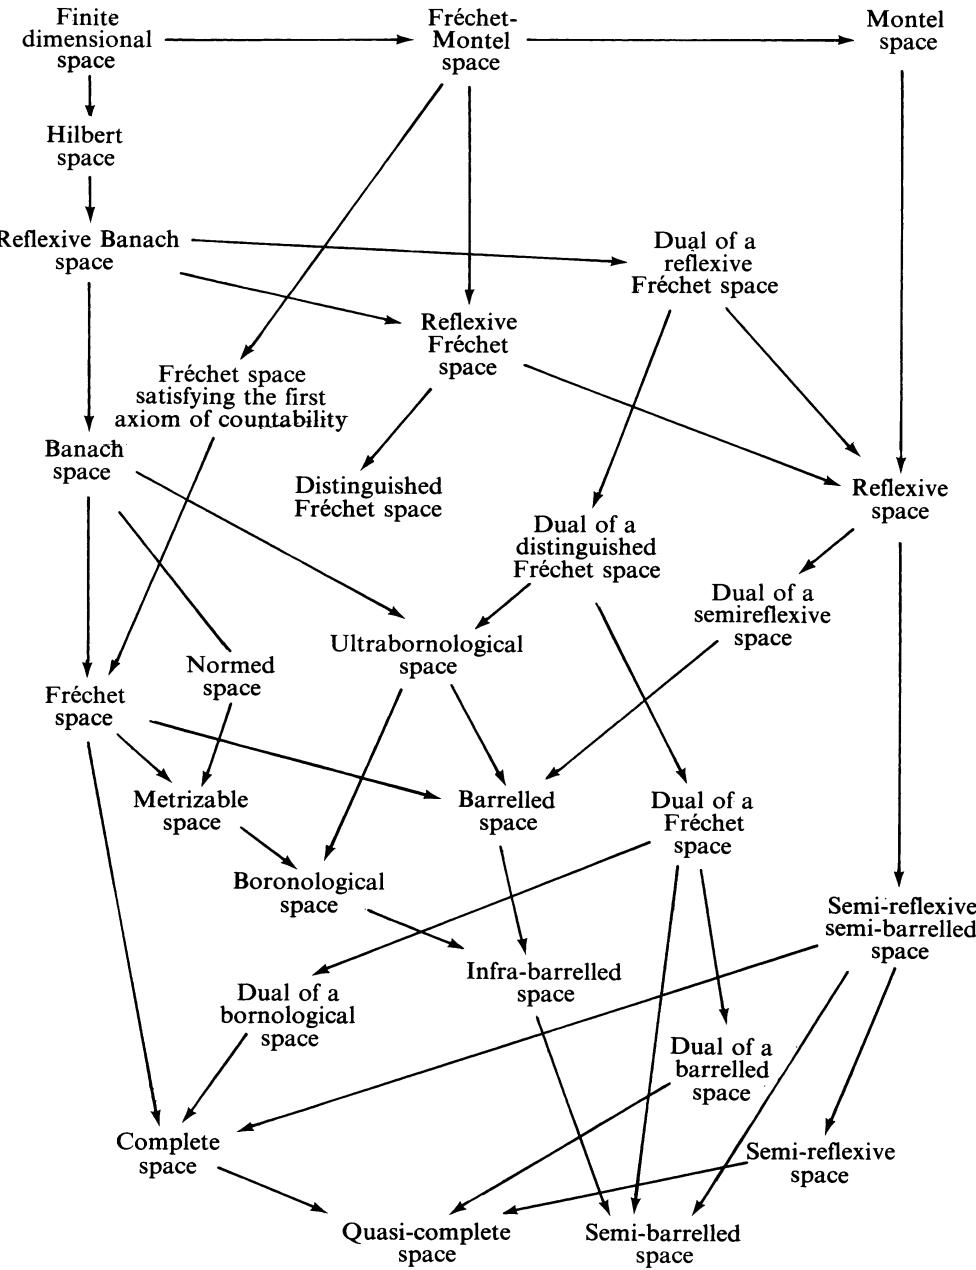
\includegraphics[keepaspectratio]{images/part002_27b26067.jpg}}

\bourbakitable{局部凸空间的对偶上的主要有界结构}{}
\pandocbounded{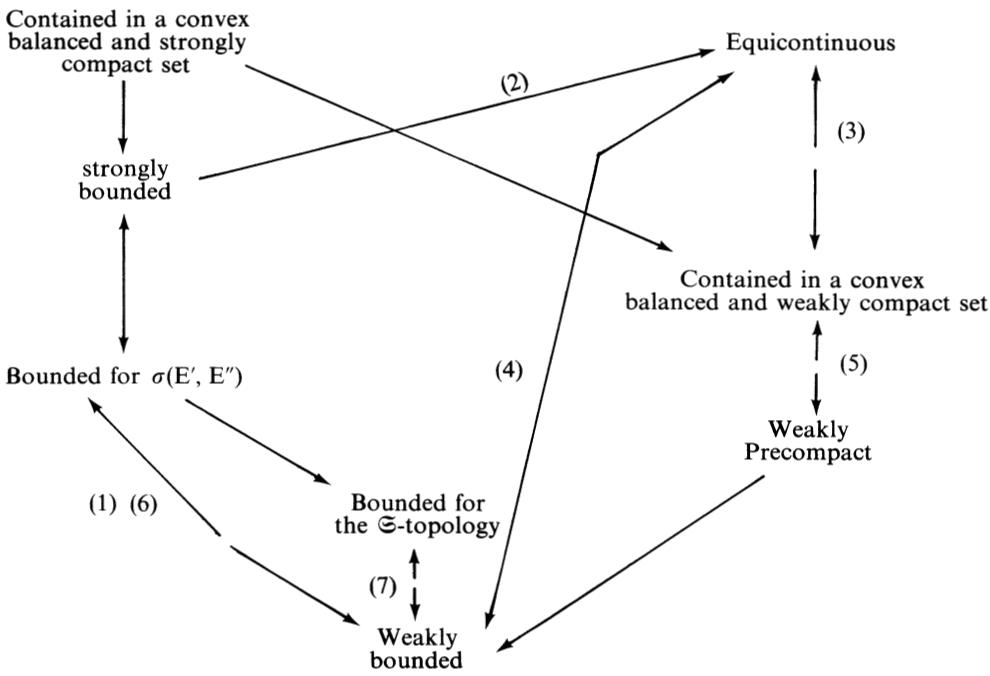
\includegraphics[keepaspectratio]{images/part002_d08e803b.jpg}}

注意 --- 我们用 S 表示 E 的有界子集的这样一个族：其每个元素都含于该族中的某个集合内。箭头旁的数字表示：当同号性质成立时，相应的蕴含关系成立。

\paragraph{性质}

\begin{enumerate}
\def\labelenumi{\arabic{enumi})}
\item
  每当 E 半自反时；
\item
  每当 E 是有界型空间时（III, p.~22, 命题 10）；
\item
  当且仅当 E 具有 Mackey 拓扑 \(\tau(\mathrm{E},\mathrm{E}^{\prime})\) ；
\item
  当且仅当 E 是桶型空间；
\item
  当且仅当 \(\mathbf{E}'\) 对 \(\sigma (\mathbf{E}',\mathbf{E})\) 拟完备
\item
  每当 E 半完备时（更不用说拟完备或完备了）（III, p.~27, 推论 1）；
\item
  每当 \(\mathfrak{S}\) 由闭凸均衡包为半完备的集合组成时（III, p.~27, 定理 2）。
\end{enumerate}

当 E 是 Montel 空间时，上述所有有界结构都相同。

